\ifdefined\mainfile\else
\documentclass{article}
\usepackage{graphicx}
\usepackage{float}
\usepackage{amsmath}
\usepackage{amssymb}
\usepackage[a4paper, left=2.5cm, right=2.5cm, top=2.5cm, bottom=2.5cm]{geometry}
\usepackage[colorlinks=true,linkcolor=black,citecolor=blue,urlcolor=blue]{hyperref}
\usepackage{tikz}
\usetikzlibrary{automata, positioning, arrows, calc}

\tikzset{
	->,
	>=stealth,
	shorten >=2pt, shorten <=2pt,
	node distance=2.8cm,
	every state/.style={draw=blue!55,very thick,fill=blue!20},
	initial text=$ $,
}

\begin{document}
\fi

\section{Syntese og Simulering}
\label{sec:synthesis}

\subsection{IDC Simulering}
\label{sec:synthesis-idc}

IDC testbenchen er opdelt i fire grupper (se testmetode i sektion~\ref{sec:idc-test}).
Nedenfor vises bølgeformerne fra Vivado XSim for hver gruppe.

\subsubsection{Gruppe 1: Register-Register Instruktioner}

Tester alle ti register-register operationer (MOVA, INC, ADD, SUB, DEC, OR, AND, XOR, NOT, MOVB).
For hver instruktion verificeres at FS matcher den forventede funktionskode,
at RW=1 (register write), og at PS=01 (PC increment).

\begin{figure}[H]
    \centering
    
\includegraphics[width=\linewidth]{images/syntese/idc_tb_group1.png}
    \caption{Simulering af Gruppe 1: Register-register operationer.
             IR skifter opcode for hver instruktion, og FS følger med den korrekte funktionskode.}
    \label{fig:idc-tb-g1}
\end{figure}

\subsubsection{Gruppe 2: Memory \& Immediate}

Tester LD, ST, ADI og LDI. Verificerer korrekt MD (memory data select),
MW (memory write), MB (MUX B for immediate operander) og FS.

\begin{figure}[H]
    \centering
    
\includegraphics[width=\linewidth]{images/syntese/idc_tb_group2.png}
    \caption{Simulering af Gruppe 2: Memory og immediate instruktioner.}
    \label{fig:idc-tb-g2}
\end{figure}

\subsubsection{Gruppe 3: Branch \& Jump}

Tester BRZ (branch on zero), BRN (branch on negative) og JMP.
For branch-instruktionerne testes både taget og ikke-taget tilfælde
ved at variere Z- og N-flag.

\begin{figure}[H]
    \centering
    
\includegraphics[width=\linewidth]{images/syntese/idc_tb_group3.png}
    \caption{Simulering af Gruppe 3: Branch og jump instruktioner.
             PS skifter mellem 10 (branch taget) og 01 (ikke taget).}
    \label{fig:idc-tb-g3}
\end{figure}

\subsubsection{Gruppe 4: Multi-cycle (LRI, SRM, SLM)}

Tester flercyklus-instruktionerne. LRI verificerer 3-cyklus forløbet
(EX0: load til R8, EX1: load fra R8-adresse). SRM/SLM tester
shift-løkken inklusive tidlig afslutning ved Z=1 og korrekt
gennemløb af EX2$\leftrightarrow$EX3 løkken.

\begin{figure}[H]
    \centering
    
\includegraphics[width=\linewidth]{images/syntese/idc_tb_group4.png}
    \caption{Simulering af Gruppe 4: Multi-cycle instruktioner.
             Bemærk de ekstra tilstande EX1--EX4 for SRM/SLM.}
    \label{fig:idc-tb-g4}
\end{figure}

\subsubsection{Verifikationsresultat}

Alle fire testgrupper blev kørt i Vivado XSim. Ingen \texttt{Error}-beskeder
blev rapporteret, hvilket bekræfter at samtlige 24 assert-statements bestod.

\begin{table}[H]
\centering
\begin{tabular}{|c|l|c|c|}
\hline
\textbf{Gruppe} & \textbf{Beskrivelse} & \textbf{Antal tests} & \textbf{Resultat} \\
\hline
1 & Register-register  & 10 & PASSED \\
2 & Memory \& Immediate    & 4  & PASSED \\
3 & Branch \& Jump         & 5  & PASSED \\
4 & Multi-cycle (LRI, SRM, SLM) & 5 & PASSED \\
\hline
  & \textbf{Total}         & \textbf{24} & \textbf{PASSED} \\
\hline
\end{tabular}
\caption{Testresultater for IDC testbench. Alle grupper bestod uden fejl.}
\label{tab:idc-test-results}
\end{table}

\subsection{MPC Top-Level Simulering}
\label{sec:synthesis-mpc}

MPC topmodulets testbench verificerer det samlede samspil mellem alle submoduler.
Testbenchen er opdelt i fire grupper (se testmetode i sektion~\ref{sec:mpc-test}).

\subsubsection{Gruppe 1: Register-Register Instruktioner}

Tester alle ti register-register operationer gennem hele signalkæden: \texttt{Instruction\_In} $\rightarrow$ IR $\rightarrow$ IDC $\rightarrow$ kontrolsignaler. For hver instruktion verificeres at FS, RW, DX og AX er korrekte, at \texttt{Constant\_Out} matcher Zero Fillerens output, og at \texttt{Address\_Out} (PC) inkrementeres efter hver instruktion.

\begin{figure}[H]
    \centering
    
\includegraphics[width=\linewidth]{images/syntese/mpc_tb_group1.png}
    \caption{Simulering af MPC Gruppe 1: Register-register instruktioner. Address\_Out inkrementeres fra 00 til 0A gennem ti instruktioner.}
    \label{fig:mpc-tb-g1}
\end{figure}

\subsubsection{Gruppe 2: Memory \& Immediate}

Tester LD, ST, ADI og LDI gennem topmodulet. Verificerer at MB=1 for immediate-instruktioner, at \texttt{Constant\_Out} indeholder det korrekte zero-filled konstantfelt, og at PC inkrementeres.

\begin{figure}[H]
    \centering
    
\includegraphics[width=\linewidth]{images/syntese/mpc_tb_group2.png}
    \caption{Simulering af MPC Gruppe 2: Memory og immediate instruktioner.}
    \label{fig:mpc-tb-g2}
\end{figure}

\subsubsection{Gruppe 3: Branch \& Jump}

Tester branch- og jump-instruktioner med fokus på \texttt{Address\_Out}-verifikation. BRZ med Z=1 udfører branch med Sign Extender-offset (PC $\leftarrow$ PC + 3 = 03). BRZ med Z=0 inkrementerer normalt. BRN med N=1 brancher (PC $\leftarrow$ PC + 10 = 0E). JMP loader \texttt{Address\_In} = 42 direkte i PC. Efterfølgende MOVA bekræfter at PC fortsat inkrementerer normalt efter jump (43).

\begin{figure}[H]
    \centering
    
\includegraphics[width=\linewidth]{images/syntese/mpc_tb_group3.png}
    \caption{Simulering af MPC Gruppe 3: Branch og jump. Address\_Out følger sekvensen 00 $\rightarrow$ 03 $\rightarrow$ 04 $\rightarrow$ 0E $\rightarrow$ 0F $\rightarrow$ 42 $\rightarrow$ 43.}
    \label{fig:mpc-tb-g3}
\end{figure}

\subsubsection{Gruppe 4: Multi-cycle}

Tester flercyklus-instruktionerne LRI, SRM og SLM. Verificerer at \texttt{Address\_Out} holdes konstant under hele flercyklus-forløbet og først inkrementeres ved afslutning. SRM med Z=0 gennemløber den fulde shift-løkke (EX0 $\rightarrow$ EX1 $\rightarrow$ EX2 $\leftrightarrow$ EX3 $\rightarrow$ EX4 $\rightarrow$ INF) mens PC forbliver uændret.

\begin{figure}[H]
    \centering
    
\includegraphics[width=\linewidth]{images/syntese/mpc_tb_group4.png}
    \caption{Simulering af MPC Gruppe 4: Multi-cycle instruktioner. Address\_Out holder sin værdi under flercyklus-forløb.}
    \label{fig:mpc-tb-g4}
\end{figure}

\subsubsection{Verifikationsresultat}

Alle fire testgrupper blev kørt i Vivado XSim. Ingen \texttt{Error}-beskeder blev rapporteret.

\begin{table}[H]
\centering
\begin{tabular}{|c|l|c|c|}
\hline
\textbf{Gruppe} & \textbf{Beskrivelse} & \textbf{Antal tests} & \textbf{Resultat} \\
\hline
1 & Register-register  & 10 & PASSED \\
2 & Memory \& Immediate    & 4  & PASSED \\
3 & Branch \& Jump         & 5  & PASSED \\
4 & Multi-cycle (LRI, SRM, SLM) & 5 & PASSED \\
\hline
  & \textbf{Total}         & \textbf{24} & \textbf{PASSED} \\
\hline
\end{tabular}
\caption{Testresultater for MPC top-level testbench. Alle grupper bestod uden fejl.}
\label{tab:mpc-test-results}
\end{table}

\subsection{Verificering af Timing Diagram}

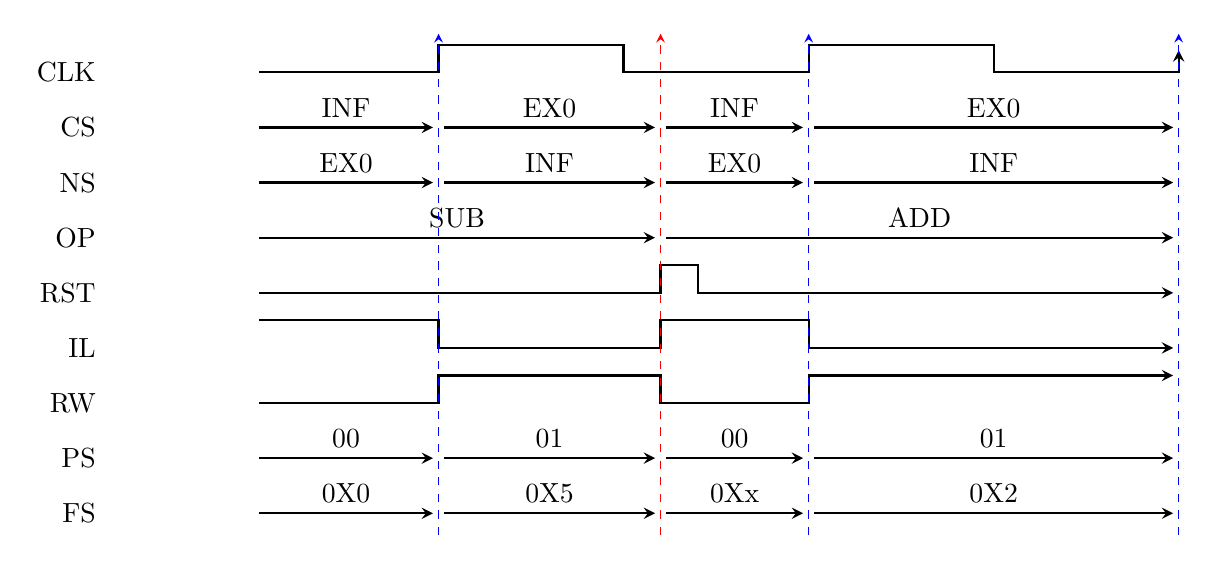
\begin{tikzpicture}[
    x=4.7cm,
    y=0.7cm,
    sig/.style={draw, thick},
    bus/.style={draw, thick},
    lbl/.style={anchor=east}
]

% --- Labels ---
\node[lbl] at (-0.4, 0) {CLK};
\node[lbl] at (-0.4,-1) {CS};
\node[lbl] at (-0.4,-2) {NS};
\node[lbl] at (-0.4,-3) {OP};
\node[lbl] at (-0.4,-4) {RST};
\node[lbl] at (-0.4,-5) {IL};
\node[lbl] at (-0.4,-6) {RW};
\node[lbl] at (-0.4,-7) {PS};
\node[lbl] at (-0.4,-8) {FS};

% --- CLK (rising edges at x = 1,2,3) ---
\draw[sig]
(0,0) -- (0.5,0) -- (0.5,0.5) -- (1,0.5) -- (1,0)
-- (1.5,0) -- (1.5,0.5) -- (2,0.5) -- (2,0)
-- (2.5,0) -- (2.5,0.5);

% CS: INF -> EX0 -> INF
\draw[bus] (0,-1) -- (0.5,-1) node[midway,above] {INF};

\draw[bus] (0.5,-1) -- (1.1,-1) node[midway,above] {EX0};

\draw[bus] (1.1,-1) -- (1.5,-1) node[midway,above] {INF};

\draw[bus] (1.5,-1) -- (2.5,-1) node[midway,above] {EX0};

% --- NS (next_state) ---
\draw[bus] (0,-2) -- (0.5,-2) node[midway,above] {EX0};

\draw[bus] (0.5,-2) -- (1.1,-2) node[midway,above] at (0.8,-2) {INF};

\draw[bus] (1.1,-2) -- (1.5,-2) node[midway,above] {EX0};

\draw[bus] (1.5,-2) -- (2.5,-2) node[midway,above] {INF};


% --- OP (konstant) ---
\draw[bus] (0,-3) -- (1.1,-3) node[midway,above] {SUB};

\draw[bus] (1.1,-3) -- (2.5,-3) node[midway,above] {ADD};

% --- RST (kort puls før start) ---
\draw[sig]
(0,-4) -- (1.1,-4) -- (1.1,-3.5) -- (1.2,-3.5) -- (1.2,-4) -- (2.5,-4);

% --- IL (høj i INF) ---
\draw[sig]
(0,-4.5) -- (0.5,-4.5) -- (0.5,-5) -- (1.1,-5) -- (1.1,-4.5) -- (1.5,-4.5) -- (1.5,-5) -- (2.5,-5);

% --- RW (høj i EX0) ---
\draw[sig]
(0,-6) -- (0.5,-6) -- (0.5,-5.5) -- (1.1,-5.5) -- (1.1,-6) -- (1.5,-6) -- (1.5,-5.5) -- (2.5,-5.5);

% --- PS ---
\draw[bus] (0,-7) -- (0.5,-7) node[midway,above] {00};

\draw[bus] (0.5,-7) -- (1.1,-7) node[midway,above] at (0.8,-7) {01};

\draw[bus] (1.1,-7) -- (1.5,-7) node[midway,above] {00};

\draw[bus] (1.5,-7) -- (2.5,-7) node[midway,above] {01};

% --- FS ---
\draw[bus] (0,-8) -- (0.5,-8) node[midway,above] {0X0};

\draw[bus] (0.5,-8) -- (1.1,-8) node[midway,above] at (0.8,-8) {0X5};

\draw[bus] (1.1,-8) -- (1.5,-8) node[midway,above] {0Xx};

\draw[bus] (1.5,-8) -- (2.5,-8) node[midway,above] {0X2};

% --- Rising edge marker ---
\draw[dashed, red] (1.1,-8.5) -- (1.1,0.8);

% --- clk edge marker ---
\draw[dashed, blue] (0.5,-8.5) -- (0.5,0.8);
\draw[dashed, blue] (1.5,-8.5) -- (1.5,0.8);
\draw[dashed, blue] (2.5,-8.5) -- (2.5,0.8);
\end{tikzpicture}
\\
\noindent
For at verificere det viste timingdiagram for IDC'en
er der udarbejdet en dedikeret VHDL testbench, som tester
\texttt{SUB}, \texttt{reset} og \texttt{ADD}.
\\
\\
\noindent
Simuleringen bekræfter, at reset korrekt tvinger FSM’en tilbage
i INF-tilstanden (kan ses på \texttt{IL}),
og at efterfølgende instruktioner udføres med korrekt timing for
IL, RW, PS og FS i overensstemmelse med timingdiagrammet.
Simuleringen kan ikke direkte følge \texttt{current\_state} og
\texttt{next\_state}, da disse er enum-variabler.
Tilstandene kan derfor ikke verificeres direkte, men de observerede
kontrolsignaler understøtter, at IDC’en befinder sig i den forventede tilstand.

\begin{figure}[H]
    \centering
    
\includegraphics[width=1\linewidth]{images/syntese/TB_af_timingdiagram.png}
    \caption{Billedet viser simulerings resultaterne af Timingdigram\_TB}
    \label{fig:TB_testdiagram}
\end{figure}
\ifdefined\mainfile\else
\end{document}
\fi
